\subsection{Determinação do calor específico de um metal}

Após a realização de todos os passos conforme dito na metodologia, pudemos obter todos os dados necessários para fazer os cálculos. Então, baseado nas informações fornecidas pelos vídeos, temos que:

\begin{table}[H]
    \centering
    \begin{tabular}{ |c||c||c||c| }
        \hline
        \textbf{O que foi medido} & \textbf{Valor} & \textbf{Incerteza} & \textbf{Unidade}\\
        \hline 
        Massa água ($m_1$) & 216,07 & $\pm$ 0,01 & g \\
        Massa do metal ($m_2$) & 205,75 & $\pm$ 0,01 & g \\
        \hline
        Temperatura calorímetro ($T_1$) & 13,1 & $\pm$ 0,1 & ºC \\
        Temperatura metal ($T_2$) & 97,1 & $\pm$ 0,1 & ºC \\
        Temperatura equilíbrio ($T_f$) & 19,2 & $\pm$ 0,1 & ºC \\
        \hline
        \end{tabular}
    \caption{Dados experimentais do experimento 2} 
\end{table}

Além dos dados obtidos experimentalmente, é necessário utilizar o valor da capacidade térmica do calorímetro deduzida anteriormente:

\[ C = 18,25 \ \ cal/^\circ C \]

Com essas informações em mãos, podemos então realizar os cálculos necessários seguindo as fórmulas deduzidas anteriormente:

\[ N = (m_1 + C) \cdot \Delta T_{f1} \]
\[ N = (216,07 + 18,25) \cdot (19,2 - 13,1) \]
\[ N = 1429,352 \]

\[ D = m_2 \cdot \Delta T_{f2} \]
\[ D = 205,75 \cdot \Delta (19,2 - 97,1) \]
\[ D = 16027,925 \]

\[ c_m = \frac{N}{D} \]
\[ c_m = \frac{1429,352}{16027,925} \]
\[ c_m = - 0,089178855 \ \ cal/g^\circ C \]

E propagando as incertezas:

\[ \delta \Delta T_{f1} = \delta T_1 + \delta T_f \]
\[ \delta \Delta T_{f1} = 0,1 + 0,1 = 0,2 \]

\[ \delta \Delta T_{f2} = \delta T_2 + \delta T_f \]
\[ \delta \Delta T_{f2} = 0,1 + 0,1 = 0,2 \]

\[ \delta N = [(m_1 + C) \cdot \delta \Delta T_{f1}] + [(\delta m_1 + \delta C) \cdot \Delta T_{f1}] \]
\[ \delta N = [(216,07 + 18,25) \cdot (0,2)] + [(0,01 + \delta C) \cdot (19,2 - 13,1)] \]
\[ \delta N = xxx \]

\[ \delta D = (\delta m_2 \cdot \Delta T_{f2}) + (m_2 \cdot \delta \Delta T_{f2}) \]
\[ \delta D = [0,2 \cdot (19,2 - 97,1)] + (205,75 \cdot 0,2) \]
\[ \delta D = yyy \]

\[ \delta c_m = \frac{N \cdot \delta D + \delta N \cdot D}{D^2} \]
\[ \delta c_m = \frac{1429,352 \cdot yyy + \delta N \cdot 16027,925}{16027,925^2} \]
\[ \delta c_m = zzzz \]

Dessa forma, podemos tomar o módulo dos valores calculados, pois uma capacidade negativa não existe, e nesse caso ela só ficou dessa forma pois o metal perdeu calor (então o seu termo na equação do equilíbrio sai negativo). Então, temos que a capacidade calorífica desse metal desconhecido vale:

\[ \mathbf{c_m = 0,089178855 \pm zzzz } \]

Comparando com os valores tabelados, podemos dizer que o valor se encontra muito próximo do Cobre ($c_{cu} = 0,093$) e também da liga metálica Latão ($c_{l} = 0,092$). Porém, além dos detalhes tabelados temos outro elemento muito importante nessa dedução: a cor do metal. Como podemos ver no vídeo, ela é bem laranja escuro, o que parece muito cobre com uma camada de óxido na sua superfície.

\begin{figure}[H]
  \centering
  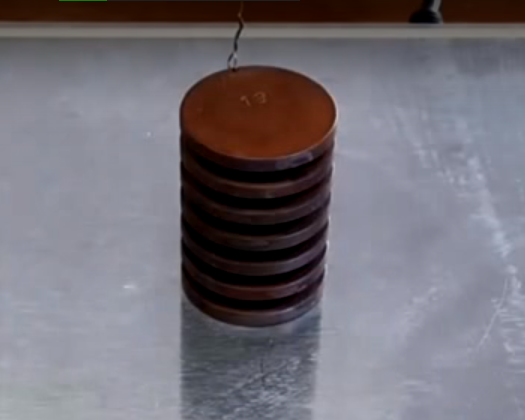
\includegraphics[scale=0.6]{images/metal.png}
  \caption{Aproximação no vídeo focando no pedaço de metal desconhecido.}
\end{figure}

Então, dito tudo isso, podemos afirmar com grande certeza de que o metal utilizado no experimento é um pedaço de \textbf{Cobre}.\\

Utilizando então o valor de $c_{cu}$ como referência, podemos notar que ele\\
1- se compatível = olha que legal
2- se não compativel = perda de calor por um sistema ideal, troca do calorimetro com o ar, buraco do termometro por convecção
